\documentclass[12pt,a4paper]{article}

% -----------------------------------------------------------------------
% Paquetes
% -----------------------------------------------------------------------
\usepackage[spanish,es-tabla]{babel}
\usepackage[utf8]{inputenc}
\usepackage[T1]{fontenc}
\usepackage{geometry}
\usepackage{graphicx}
\usepackage{booktabs}
\usepackage{amsmath}
\usepackage{amssymb}
\usepackage[hidelinks]{hyperref}
\usepackage{float}
\usepackage{caption}
\usepackage{subcaption}
\usepackage{array}
\usepackage{longtable}
\usepackage{xcolor}
\usepackage{fancyhdr}
\usepackage{titlesec}
\usepackage{parskip}
\usepackage{listings}
\usepackage{enumitem}
\usepackage{tabularx}
\usepackage{setspace}

% -----------------------------------------------------------------------
% Geometría
% -----------------------------------------------------------------------
\geometry{
  a4paper,
  top=2.5cm, bottom=2.5cm,
  left=3cm,  right=2.5cm,
  headheight=14.5pt
}

% -----------------------------------------------------------------------
% Encabezado / pie
% -----------------------------------------------------------------------
\pagestyle{fancy}
\fancyhf{}
\fancyhead[L]{\small Simulación Muelle Turístico -- Puno}
\fancyhead[R]{\small SIS230 -- UNAP}
\fancyfoot[C]{\thepage}
\renewcommand{\headrulewidth}{0.4pt}

% -----------------------------------------------------------------------
% Código fuente
% -----------------------------------------------------------------------
\definecolor{codebg}{RGB}{248,248,252}
\definecolor{codeframe}{RGB}{200,200,215}
\definecolor{codekw}{RGB}{0,80,160}
\definecolor{codecomment}{RGB}{80,130,80}
\definecolor{codestr}{RGB}{180,70,20}
\definecolor{codenum}{RGB}{130,130,140}

\lstset{
  language=Python,
  basicstyle=\ttfamily\footnotesize,
  keywordstyle=\color{codekw}\bfseries,
  commentstyle=\color{codecomment}\itshape,
  stringstyle=\color{codestr},
  showstringspaces=false,
  breaklines=true,
  breakatwhitespace=true,
  frame=single,
  rulecolor=\color{codeframe},
  backgroundcolor=\color{codebg},
  numbers=left,
  numberstyle=\tiny\color{codenum},
  numbersep=10pt,
  xleftmargin=2.5em,
  framexleftmargin=2.5em,
  aboveskip=0.9em,
  belowskip=0.9em,
  tabsize=4,
  keepspaces=true,
  columns=flexible,
}

% -----------------------------------------------------------------------
% Interlineado
% -----------------------------------------------------------------------
\setstretch{1.15}

% -----------------------------------------------------------------------
% Metadata PDF
% -----------------------------------------------------------------------
\hypersetup{
  pdftitle={Simulación Montecarlo del Sistema de Embarcaciones Turísticas -- Lago Titicaca},
  pdfauthor={Rendo Alfonte Tarqui, Yimmy Yeyson Cuyo Zamata, Cristian Alexis Loza Torres},
  pdfsubject={SIS230 Modelado Sistémico y Simulación},
}

% =======================================================================
\begin{document}
% =======================================================================

% -----------------------------------------------------------------------
% PORTADA
% -----------------------------------------------------------------------
\begin{titlepage}
  \centering
  \vspace*{0.5cm}

  % Logos institucionales
  \begin{minipage}{0.35\textwidth}
    \centering
    
\includegraphics[width=3.2cm]{logos/Logo_UNAP.png}
  \end{minipage}
  \hfill
  \begin{minipage}{0.35\textwidth}
    \centering
    \includegraphics[width=3.2cm]{logos/Sistemas.png}
  \end{minipage}

  \vspace{0.6cm}
  {\large\bfseries Universidad Nacional del Altiplano -- Puno}\\[0.3cm]
  {\normalsize Facultad de Ingeniería Mecánica, Eléctrica, Electrónica y Sistemas}\\[0.2cm]
  {\normalsize Escuela Profesional de Ingeniería de Sistemas}\\[1.5cm]

  \rule{\linewidth}{0.8pt}\\[0.5cm]
  {\Large\bfseries Simulación Montecarlo de distribuciones continuas\\[0.3cm]
  para la optimización del sistema de embarcaciones\\[0.3cm]
  turísticas en el Lago Titicaca, Puno}\\[0.5cm]
  \rule{\linewidth}{0.8pt}\\[1.2cm]

  % Tabla de detalles
  \begin{tabular}{ll}
    \toprule
    \textbf{Categoría} & \textbf{Información} \\
    \midrule
    Asignatura & SIS230 -- MODELADO SISTÉMICO Y SIMULACIÓN \\
    Docente    & Dr.\ Ing.\ FLORES VELASQUEZ EDELFRE \\
    \bottomrule
  \end{tabular}\\[1.2cm]

  {\bfseries Presentado por el Estudiante:}\\[0.5cm]
  \begin{tabular}{ll}
    \toprule
    \textbf{Código Universitario} & \textbf{Nombres y Apellidos} \\
    \midrule
    228526 & Rendo Alfonte Tarqui \\
    229425 & Yimmy Yeyson Cuyo Zamata \\
    227329 & Cristian Alexis Loza Torres \\
    \bottomrule
  \end{tabular}\\[1.5cm]

  \raggedleft
  Semestre 2026~--~I\\
  Puno~--~Perú\\[0.3cm]
  {\bfseries 29 may 2026}

\end{titlepage}

% -----------------------------------------------------------------------
% ÍNDICE
% -----------------------------------------------------------------------
\tableofcontents
\newpage

% -----------------------------------------------------------------------
% 1. RESUMEN
% -----------------------------------------------------------------------
\section{Resumen}

El presente trabajo implementa una simulación Montecarlo del sistema de
embarcaciones turísticas del Muelle Turístico de Puno, que opera hacia las
islas del Lago Titicaca. El sistema presenta variabilidad en llegada de
grupos turísticos, registro, disponibilidad de embarcaciones, navegación y
permanencia en destino. Se modelaron cinco variables aleatorias con
distribuciones Exponencial, Triangular y Uniforme, y se ejecutaron 1\,000
réplicas Montecarlo por escenario. Los resultados del escenario base
revelan una espera promedio de \textbf{66,2 minutos} desde la llegada
hasta el embarque, con una utilización de embarcaciones del \textbf{82,8\%}
y aproximadamente \textbf{225 turistas no atendidos} por jornada de cuatro
horas. Se compararon cuatro escenarios alternativos: agregar una
embarcación (E1), reducir el tiempo de preparación (E2), aumentar la
capacidad (E3) y simular alta demanda (E4). Los escenarios E1 y E3
muestran las mejoras más significativas; E2 ofrece un impacto marginal
dado que el tiempo de preparación representa menos del 6\% del ciclo total.
Se recomienda implementar E1 como acción prioritaria y E3 como alternativa
de mayor eficiencia por viaje.

\newpage

% -----------------------------------------------------------------------
% 2. INTRODUCCIÓN
% -----------------------------------------------------------------------
\section{Introducción}

Puno es uno de los destinos turísticos más importantes del Perú por su
valor cultural, festivo y natural. El Lago Titicaca, con una extensión de
8\,562 km², es el lago navegable más alto del mundo y atrae a cientos de
miles de turistas cada año, especialmente durante la Festividad de la
Virgen de la Candelaria, declarada Patrimonio Cultural Inmaterial de la
Humanidad por la UNESCO.

El Muelle Turístico de Puno concentra las operaciones de embarque hacia
las Islas Flotantes de los Uros, Taquile y Amantaní. La demanda turística
es estacional e irregular: los grupos llegan de manera variable, los
tiempos de registro dependen del tipo de grupo, y la disponibilidad de
embarcaciones está limitada por el tiempo de ciclo completo que incluye
navegación de ida, permanencia en la isla, retorno y preparación del bote.

Sin un modelo cuantitativo, no es posible anticipar cuántos turistas
quedarán sin ser atendidos en una jornada pico, ni qué mejora operativa
conviene adoptar. La simulación Montecarlo permite reproducir el
comportamiento estocástico del sistema miles de veces, calcular métricas
de desempeño y comparar escenarios de mejora antes de tomar decisiones que
afecten la operación real.

Este trabajo diseña, implementa y analiza dicha simulación usando Python con
las bibliotecas NumPy, Pandas, Matplotlib y Seaborn. El alcance cubre la
jornada de mayor demanda (06:00 a 10:00), con 3 embarcaciones base y
capacidad para 30 turistas por embarcación.

% -----------------------------------------------------------------------
% 3. CONTEXTO REAL DEL TURISMO EN PUNO
% -----------------------------------------------------------------------
\section{Contexto real del turismo en Puno y Lago Titicaca}

\subsection{Importancia turística}

Según datos del Ministerio de Comercio Exterior y Turismo (MINCETUR) para
la Festividad de la Virgen de la Candelaria 2026, Puno recibió
\textbf{92\,960 turistas} con un impacto económico estimado de
\textbf{S/~117,6 millones}. Del total de visitantes:

\begin{itemize}[noitemsep]
  \item El 75,6\% visitó el Lago Titicaca.
  \item El 44,9\% visitó las Islas Flotantes de los Uros.
  \item El 14,4\% visitó la Isla Taquile.
  \item El 60,7\% llegó en bus interprovincial.
  \item El 23,2\% llegó por vía aérea.
\end{itemize}

\subsection{Marco institucional y ambiental}

El Ente Gestor Destino Lago Titicaca, dependiente de MINCETUR, gestiona 57
atractivos turísticos secundarios en la cuenca. El lago está protegido como
Reserva Nacional del Titicaca (SERNANP), lo que impone regulaciones de
capacidad de carga y seguridad en la operación de embarcaciones.

\subsection{Referencia operativa}

El operador PunoTours publica tours de Uros y Taquile con salida desde el
muelle a las 07:15 y retorno a las 16:00. Esto confirma que el ciclo
completo puede extenderse más allá de la jornada de embarque y que la
disponibilidad de embarcaciones en las primeras horas es el cuello de
botella principal del sistema.

% -----------------------------------------------------------------------
% 4. PLANTEAMIENTO DEL PROBLEMA
% -----------------------------------------------------------------------
\section{Planteamiento del problema}

El Muelle Turístico de Puno opera con un número fijo de embarcaciones cuyo
ciclo de servicio es largo: cada viaje incluye navegación de ida (25--40
min), permanencia en isla (45--180 min), retorno (25--40 min) y
preparación (10 min). Durante ese ciclo, los turistas continúan llegando y
el sistema acumula cola.

\medskip
Las principales fuentes de variabilidad son:

\begin{enumerate}[noitemsep]
  \item Tiempo entre llegadas de grupos turísticos.
  \item Tamaño de cada grupo.
  \item Tiempo de registro y pago en ventanilla.
  \item Tiempo de navegación (condiciones de viento y oleaje).
  \item Tiempo de permanencia en destino (tipo de tour).
\end{enumerate}

\medskip
Sin un modelo de simulación, los gestores del muelle no pueden responder
preguntas como: ¿cuántos turistas quedan sin ser atendidos en una jornada
pico?, ¿qué mejora operativa reduce más las esperas con menor inversión?,
¿cómo se comporta el sistema si la demanda aumenta un 25\%?

La simulación Montecarlo replica el comportamiento estocástico del sistema
1\,000 veces para cada escenario, produciendo distribuciones empíricas de
las métricas de interés y permitiendo comparaciones estadísticamente
robustas.

% -----------------------------------------------------------------------
% 5. OBJETIVOS
% -----------------------------------------------------------------------
\section{Objetivos}

\subsection{Objetivo general}

Diseñar, implementar y analizar una simulación Montecarlo del sistema de
embarcaciones turísticas del Lago Titicaca para evaluar tiempos de espera,
longitud de cola, utilización de embarcaciones y escenarios de mejora
operativa.

\subsection{Objetivos específicos}

\begin{enumerate}[noitemsep]
  \item Identificar las variables aleatorias del sistema turístico de
    embarcaciones.
  \item Definir una distribución de probabilidad para cada variable.
  \item Justificar cada distribución usando el PDF base, fuentes reales y
    una ficha de observación sintética.
  \item Generar datos sintéticos coherentes para una ventana operativa
    representativa de una hora.
  \item Implementar la simulación en un notebook Python.
  \item Validar las distribuciones mediante histogramas, medias y varianzas.
  \item Simular el escenario base durante una jornada de cuatro horas.
  \item Ejecutar 1\,000 repeticiones Montecarlo por escenario.
  \item Comparar escenarios alternativos.
  \item Recomendar la mejor alternativa operativa.
\end{enumerate}

% -----------------------------------------------------------------------
% 6. DESCRIPCIÓN DEL SISTEMA
% -----------------------------------------------------------------------
\section{Descripción del sistema}

\subsection{Flujo operativo}

Para entender cómo funciona el sistema, es importante partir desde lo más
básico: lo que ocurre cada mañana en el Muelle Turístico de Puno. Los
grupos de turistas llegan, hacen fila para registrarse, pagan su pasaje y
luego esperan hasta que una embarcación esté disponible para llevarlos a
las islas. Una vez a bordo, viajan hasta su destino, permanecen un tiempo
en la isla y finalmente regresan al muelle. Antes de recibir nuevos
pasajeros, la embarcación necesita un tiempo para alistarse nuevamente.

Todo ese proceso, desde que el grupo llega hasta que la embarcación está
lista para el siguiente viaje, se puede resumir así:

\begin{center}
\small
Llegada del grupo $\;\to\;$ Cola en ventanilla $\;\to\;$ Registro y pago
$\;\to\;$ Cola de embarque (FIFO) $\;\to\;$ Asignación a embarcación
$\;\to\;$ Navegación de ida $\;\to\;$ Permanencia en isla $\;\to\;$
Navegación de retorno $\;\to\;$ Preparación para siguiente viaje
\end{center}

La jornada que se modela abarca desde las 06:00 hasta las 10:00, es decir,
240 minutos continuos de operación.

\subsection{Entidades y recursos del sistema}

La unidad que se mueve a través del sistema no es el turista individual
sino el \textbf{grupo turístico}. Esto es importante porque los grupos no
se separan: si un grupo de 12 personas llega junto, embarca junto y se
contabiliza junto. Dividir un grupo no está permitido dentro del modelo.

Los recursos que atienden a esos grupos son dos:

\begin{description}[noitemsep]
  \item[Ventanilla de registro:] un único punto de atención donde cada
    grupo realiza el proceso de registro y pago antes de pasar a la zona
    de embarque. La disciplina es FIFO: el primero en llegar es el primero
    en ser atendido.
  \item[Embarcaciones:] en el escenario base se dispone de tres
    embarcaciones que operan en paralelo. Cada una funciona como un
    servidor independiente con capacidad para 30 turistas por viaje.
\end{description}

\subsection{Reglas de operación}

El modelo incorpora reglas concretas que determinan cuándo una embarcación
parte y qué ocurre al final de la jornada:

\begin{itemize}[noitemsep]
  \item Una embarcación zarpa cuando acumula \textbf{24 turistas o más}
    en su cola de embarque, lo que representa el 80\% de su capacidad.
  \item Si el primer grupo en cola lleva \textbf{15 minutos esperando} y
    la embarcación aún no alcanzó el umbral, parte de todas formas para
    no acumular más demora.
  \item La capacidad máxima por viaje es de \textbf{30 turistas}. Si el
    siguiente grupo en cola no cabe completo, la embarcación espera al
    siguiente grupo disponible o cumple el tiempo máximo de espera.
  \item Cuando el reloj llega a los 240 minutos (10:00), no se autoriza
    la salida de ninguna embarcación adicional. Los grupos que aún estén
    en cola quedan sin ser atendidos durante esa jornada.
\end{itemize}

% -----------------------------------------------------------------------
% 7. FICHA DE OBSERVACIÓN SINTÉTICA
% -----------------------------------------------------------------------
\section{Ficha de observación sintética}

\subsection{Justificación metodológica}

No se encontró fuente pública oficial con registros minuto a minuto del
muelle (llegadas exactas, tiempos de registro, frecuencia de salidas). Por
ello, se construyó una \textbf{ficha de observación sintética} de una hora
(09:00 a 10:00 del 29 de mayo de 2026), basada en:

\begin{itemize}[noitemsep]
  \item El PDF base del trabajo encargado.
  \item Fuentes públicas: MINCETUR, SERNANP, PunoTours.
  \item Material audiovisual referencial del flujo turístico en el muelle.
  \item Supuestos coherentes con una tasa promedio de 8 grupos/hora.
\end{itemize}

\noindent\textit{Esta ficha no se presenta como medición presencial oficial
ni como registro de campo propio del equipo. Es una construcción académica
con fines de justificación de parámetros del modelo.}

\subsection{Tabla de observación}

\begin{table}[H]
  \centering
  \caption{Ficha de observación sintética -- ventana 09:00 a 10:00 del 29 de mayo de 2026}
  \small
  \begin{tabularx}{\textwidth}{@{} c l r r r l X @{}}
    \toprule
    N\textsuperscript{o} & Hora llegada & Interll. & Tamaño & Reg. & Destino & Observación \\
     & & (min) & (tur.) & (min) & & \\
    \midrule
    1 & 09:03 & 3 &  6 & 4,1 & Uros & Grupo familiar pequeño \\
    2 & 09:10 & 7 & 12 & 5,3 & Uros & Grupo con guía local   \\
    3 & 09:18 & 8 &  8 & 3,8 & Uros & Registro rápido        \\
    4 & 09:25 & 7 & 15 & 6,2 & Uros & Pago dividido          \\
    5 & 09:34 & 9 &  4 & 3,4 & Uros & Grupo pequeño          \\
    6 & 09:40 & 6 & 18 & 6,8 & Uros & Grupo grande           \\
    7 & 09:48 & 8 & 10 & 4,7 & Uros & Grupo mixto            \\
    8 & 09:56 & 8 &  7 & 5,0 & Uros & Grupo familiar         \\
    \bottomrule
  \end{tabularx}
\end{table}

\begin{table}[H]
  \centering
  \caption{Resumen de la ventana observada}
  \begin{tabular}{@{}lr@{}}
    \toprule
    Indicador & Valor \\
    \midrule
    Grupos observados         &  8      \\
    Turistas observados       & 80      \\
    Interllegada promedio     &  7,0 min \\
    Registro promedio         &  4,9 min \\
    Tamaño promedio de grupo  & 10 turistas \\
    \bottomrule
  \end{tabular}
\end{table}

% -----------------------------------------------------------------------
% 8. VARIABLES Y DISTRIBUCIONES
% -----------------------------------------------------------------------
\section{Variables aleatorias y distribuciones}

Antes de programar cualquier simulación, es necesario decidir qué
distribución de probabilidad representa mejor cada variable del sistema.
Esta decisión no es arbitraria: cada distribución se elige porque su
forma matemática coincide con el comportamiento real o esperado del
fenómeno que modela. A continuación se presenta la tabla completa de
variables y, después, la justificación de cada elección.

\begin{table}[H]
  \centering
  \caption{Variables aleatorias del modelo de simulación}
  \small
  \begin{tabularx}{\textwidth}{@{} p{3.4cm} p{1.2cm} p{2.8cm} p{3.2cm} X @{}}
    \toprule
    Variable & Símbolo & Distribución & Parámetros & Justificación \\
    \midrule
    Tiempo entre llegadas & $T_a$ & Exponencial & $\mu = 7{,}5$ min &
      Llegadas independientes; 8 grupos/hora promedio. \\[3pt]
    Tamaño de grupo & $G$ & Triangular discreta & mín~4, moda~10, máx~18 &
      Basado en ficha de observación sintética. \\[3pt]
    Tiempo de registro & $T_r$ & Triangular & mín~3, moda~5, máx~7 &
      Proceso manual con variabilidad moderada y acotada. \\[3pt]
    Navegación ida & $T_{n1}$ & Uniforme & mín~25, máx~40 &
      Sin valor preferente dentro del rango; depende del viento. \\[3pt]
    Permanencia en isla & $T_p$ & Triangular & mín~45, moda~90, máx~180 &
      Existe un valor más frecuente con variabilidad amplia. \\[3pt]
    Navegación retorno & $T_{n2}$ & Uniforme & mín~25, máx~40 &
      Condiciones simétricas al viaje de ida. \\[3pt]
    Preparación & $T_{prep}$ & Constante & 10 min &
      Proceso estandarizado sin variabilidad observada. \\[3pt]
    Capacidad embarcación & $C$ & Constante & 30 turistas &
      Regla operativa base establecida en el PDF del trabajo. \\[3pt]
    N\textsuperscript{o} embarcaciones & $c$ & Constante & 3 &
      Configuración base del muelle turístico. \\
    \bottomrule
  \end{tabularx}
\end{table}

\subsection{Justificación de cada distribución}

\paragraph{Tiempo entre llegadas — Exponencial.}
Los grupos turísticos no llegan con un horario fijo: unos días llegan
varios en pocos minutos y otros días pasan intervalos más largos sin
nadie. Ese comportamiento, donde los eventos son independientes entre sí
y ocurren a una tasa promedio estable, es exactamente lo que modela la
distribución exponencial. Con una tasa de 8 grupos por hora, la media
entre llegadas es de 7,5 minutos.

\paragraph{Tamaño de grupo — Triangular discreta.}
La ficha de observación sintética registró grupos de entre 4 y 18
turistas, con la mayoría cerca de los 10. Cuando se conoce un mínimo,
un máximo y un valor más probable pero no se tienen suficientes datos
históricos para ajustar una distribución más compleja, la triangular
es la opción más honesta y defendible.

\paragraph{Tiempo de registro — Triangular.}
El registro es un proceso manual que depende del número de personas en
el grupo, la forma de pago y la experiencia del operador. Puede tomar
tan poco como 3 minutos en grupos pequeños con pago en efectivo o
hasta 7 minutos si hay problemas. El valor más frecuente es 5 minutos.
La triangular $\mathcal{T}(3, 5, 7)$ captura exactamente esa
variabilidad acotada.

\paragraph{Tiempo de navegación — Uniforme.}
El trayecto hacia las Islas Uros toma entre 25 y 40 minutos según las
condiciones del lago. No hay un tiempo más probable que otro dentro de
ese rango: depende del viento, el oleaje y la potencia del motor. La
distribución uniforme $\mathcal{U}(25, 40)$ es la adecuada cuando
todos los valores del intervalo son igualmente posibles.

\paragraph{Permanencia en isla — Triangular.}
Los tours tienen duraciones distintas: visitas rápidas de 45 minutos,
recorridos estándar de 90 minutos y circuitos extendidos de hasta 3
horas. El tour de 90 minutos es el más contratado, por eso es la moda.
La triangular $\mathcal{T}(45, 90, 180)$ representa bien esa
distribución con cola derecha más larga.

\subsection{Generación en Python}

\begin{lstlisting}[caption={Funciones generadoras de variables aleatorias}]
rng = np.random.default_rng(2026)

def generar_interllegada(rng, media=7.5):
    return rng.exponential(scale=media)

def generar_tamano_grupo(rng):
    return max(1, int(round(rng.triangular(left=4, mode=10, right=18))))

def generar_registro(rng):
    return rng.triangular(left=3, mode=5, right=7)

def generar_navegacion(rng):
    return rng.uniform(25, 40)

def generar_permanencia(rng):
    return rng.triangular(left=45, mode=90, right=180)
\end{lstlisting}
% -----------------------------------------------------------------------
% 9. MODELO DE SIMULACIÓN MONTECARLO
% -----------------------------------------------------------------------
\section{Modelo de simulación Montecarlo}

\subsection{¿Qué hace Montecarlo en este contexto?}

La idea central de Montecarlo es simple: en lugar de intentar resolver
el sistema con ecuaciones exactas, se simula lo que pasaría en una
jornada real muchas veces, cada vez con valores aleatorios distintos, y
se promedian los resultados. Eso es precisamente lo que hace este modelo:
repite una jornada completa de 240 minutos \textbf{1\,000 veces}, cada
una con sus propias llegadas, tamaños de grupo, tiempos de registro y
condiciones de navegación.

¿Por qué 1\,000 réplicas y no 100 o 10\,000? Porque con 1\,000 los
promedios ya son estables: agregar más réplicas no cambia
significativamente los resultados, pero reducirlas introduce demasiada
variabilidad estadística. Es un balance entre precisión y costo
computacional.

\subsection{Cómo se desarrolla cada réplica}

Cada una de las 1\,000 jornadas simuladas sigue el mismo proceso:

\begin{enumerate}[noitemsep]
  \item Se fija la semilla aleatoria \texttt{2026} para que los
    resultados sean reproducibles.
  \item Se generan los tiempos entre llegadas de grupos hasta completar
    los 240 minutos de jornada.
  \item A cada grupo se le asigna un tamaño y un tiempo de registro.
    Con eso se calcula cuándo termina de registrarse, respetando la
    cola FIFO de la ventanilla.
  \item Los grupos ordenados por fin de registro pasan a la cola de
    embarque.
  \item Se mantiene el registro de disponibilidad de cada embarcación.
  \item Cuando una embarcación queda libre, se evalúa la cola:
    \begin{enumerate}[noitemsep,label=\alph*.]
      \item Se cargan grupos en orden FIFO sin dividirlos.
      \item La embarcación parte al alcanzar 24 turistas o cuando el
        primer grupo en cola lleva 15 minutos esperando.
      \item Si la hora de salida supera los 240 minutos, la jornada
        cierra y los grupos restantes quedan sin atender.
      \item El ciclo completo de la embarcación se calcula como:
        $T_{n1} + T_p + T_{n2} + T_{prep}$.
    \end{enumerate}
  \item Para cada grupo atendido se registra su tiempo de espera:
    $W_q = t_{\text{salida}} - t_{\text{llegada}}$.
  \item Al finalizar la jornada se calculan todas las métricas.
  \item Se repite desde el paso 2 hasta completar las 1\,000 réplicas
    y se promedian los resultados.
\end{enumerate}

\subsection{Métricas calculadas}

Las métricas que se obtienen de cada réplica y se promedian al final son
las siguientes:

\begin{align}
  W_q &= \frac{1}{n}\sum_{i=1}^{n}(t_{\text{salida},i} -
    t_{\text{llegada},i})
    \tag{Espera promedio} \\[6pt]
  W   &= W_q + E[T_{n1} + T_p + T_{n2}]
    \tag{Tiempo total en sistema} \\[6pt]
  L_q &= \lambda \cdot W_q \quad (\text{Ley de Little})
    \tag{Longitud de cola} \\[6pt]
  \rho &= \frac{\sum t_{\text{activo en jornada}}}{T_{\text{jornada}}
    \cdot c}
    \tag{Utilización de embarcaciones}
\end{align}

\noindent donde $\lambda = 8/60$ grupos por minuto,
$T_{\text{jornada}} = 240$ minutos y $c$ es el número de embarcaciones
del escenario evaluado.

% -----------------------------------------------------------------------
% 10. IMPLEMENTACIÓN EN PYTHON
% -----------------------------------------------------------------------
\section{Implementación en Python}

\subsection{Entorno y librerías}

\begin{lstlisting}[caption={Importaciones y parámetros globales}]
import numpy as np
import pandas as pd
import matplotlib.pyplot as plt
import seaborn as sns

rng = np.random.default_rng(2026)

DURACION_JORNADA    = 240   # minutos
N_REPLICAS          = 1000
LAMBDA_GRUPOS_HORA  = 8
MEDIA_INTERLLEGADA  = 7.5
N_EMBARCACIONES     = 3
CAPACIDAD           = 30
UMBRAL_SALIDA       = 24
ESPERA_MAXIMA_SALIDA = 15
TIEMPO_PREPARACION  = 10
\end{lstlisting}

\subsection{Estructura del notebook}

El notebook \texttt{simulacion\_embarcaciones\_titicaca.ipynb} tiene las
siguientes secciones:

\begin{enumerate}[noitemsep]
  \item Título e introducción.
  \item Importación de librerías y parámetros.
  \item Ficha de observación sintética.
  \item Generadores de variables aleatorias.
  \item Validación de distribuciones.
  \item Generación de grupos y ventanilla FIFO.
  \item Simulación de una jornada.
  \item Simulación Montecarlo -- escenario base.
  \item Escenarios alternativos.
  \item Comparación de métricas.
  \item Gráficos finales.
  \item Conclusiones técnicas del notebook.
\end{enumerate}

% -----------------------------------------------------------------------
% 11. VALIDACIÓN DE DISTRIBUCIONES
% -----------------------------------------------------------------------
\section{Validación de distribuciones}

Se generaron \textbf{10\,000 muestras} de cada variable y se compararon
las medias muestrales con las medias teóricas.

\begin{table}[H]
  \centering
  \caption{Comparación de medias: muestral vs.\ teórica (n = 10\,000, semilla 2026)}
  \begin{tabular}{@{}lrrr@{}}
    \toprule
    Variable & Media muestral & Media teórica & Varianza muestral \\
    \midrule
    Interllegadas   &  7,6528 &  7,5000 &  57,1508 \\
    Tamaño de grupo & 10,6379 & 10,6667 &   8,2196 \\
    Registro        &  4,9850 &  5,0000 &   0,6717 \\
    Navegación ida  & 32,4513 & 32,5000 &  18,7879 \\
    Permanencia     & 104,681 & 105,000 & 784,230  \\
    \bottomrule
  \end{tabular}
\end{table}

\noindent La desviación entre media muestral y teórica es inferior al 1\%
en todos los casos, lo que confirma que los generadores producen muestras
consistentes con las distribuciones definidas.

\subsection{Histogramas de validación}

\begin{figure}[H]
  \centering
  \begin{subfigure}[b]{0.48\textwidth}
    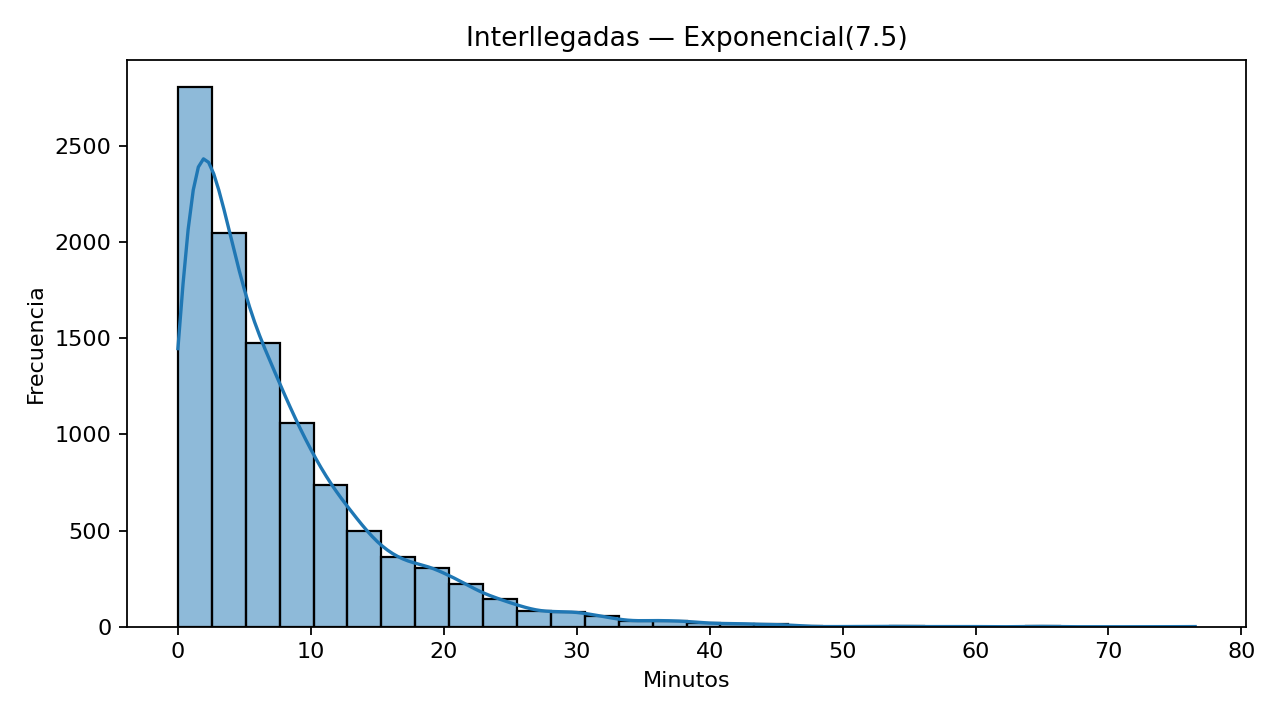
\includegraphics[width=\textwidth]{../figures/hist_interllegadas.png}
    \caption{Interllegadas -- Exponencial}
  \end{subfigure}
  \hfill
  \begin{subfigure}[b]{0.48\textwidth}
    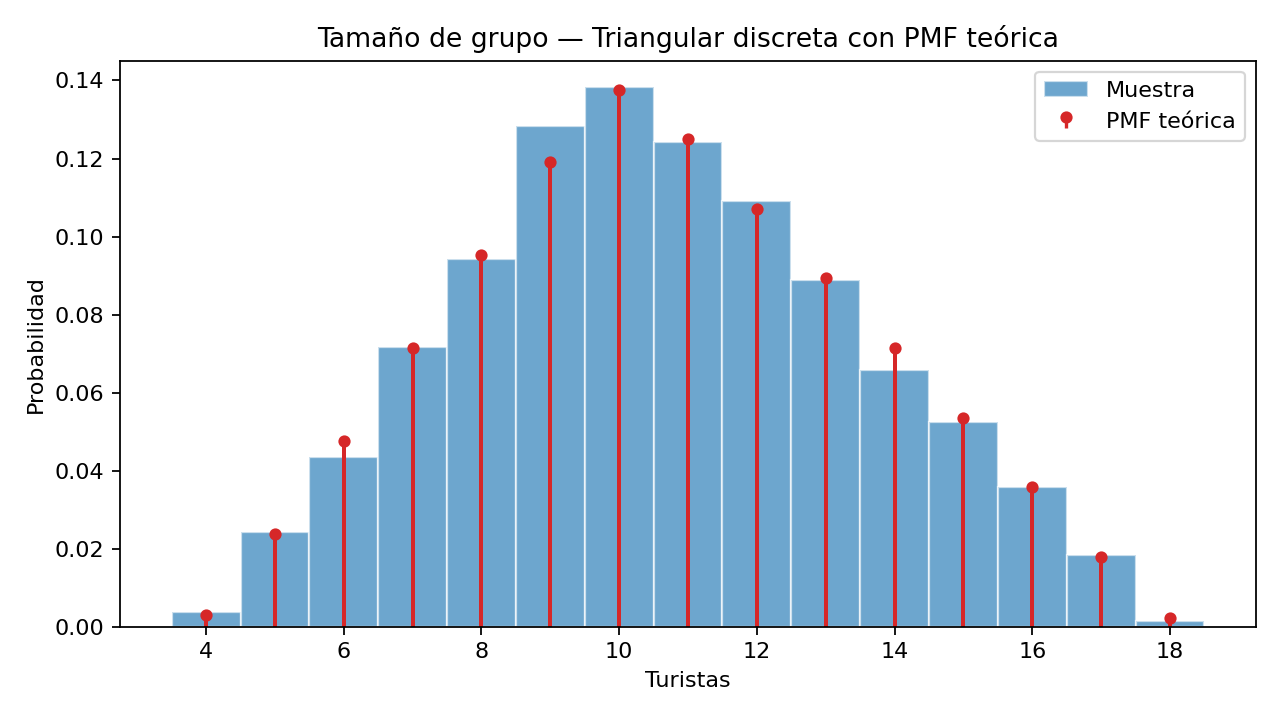
\includegraphics[width=\textwidth]{../figures/hist_tamano_grupo.png}
    \caption{Tamaño de grupo -- Triangular discreta}
  \end{subfigure}

  \vspace{0.5cm}

  \begin{subfigure}[b]{0.48\textwidth}
    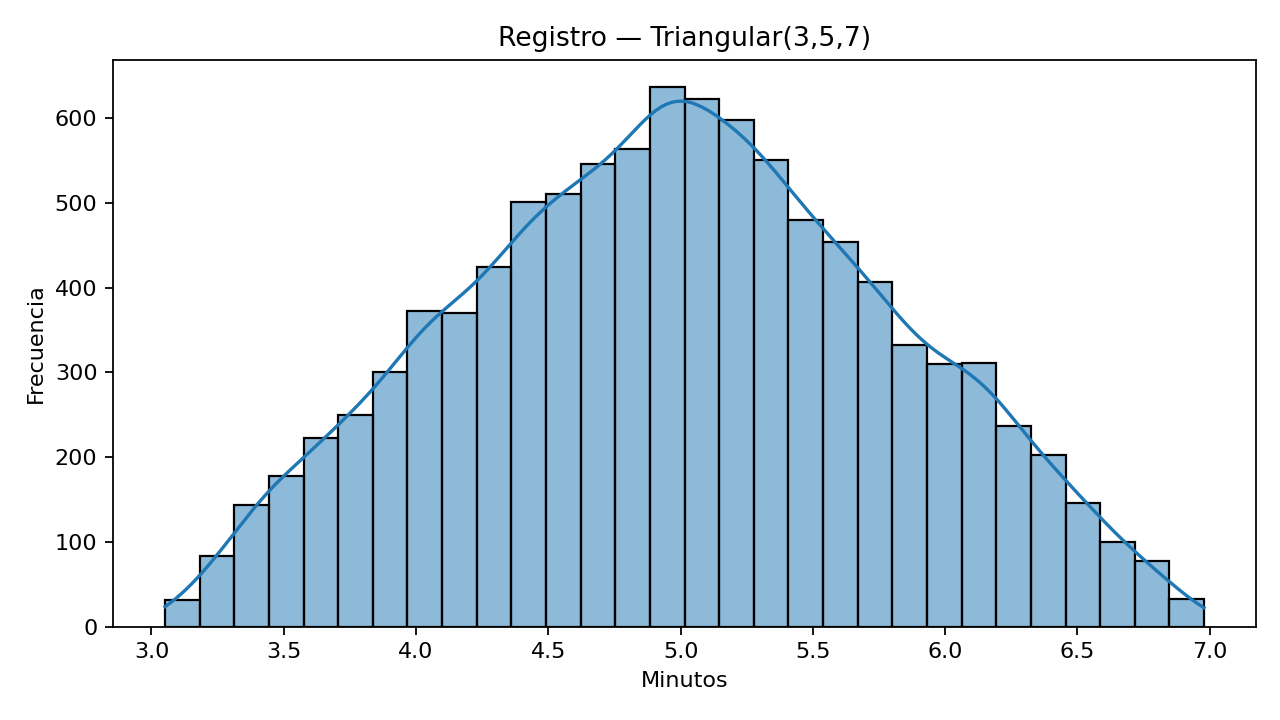
\includegraphics[width=\textwidth]{../figures/hist_registro.png}
    \caption{Registro -- Triangular}
  \end{subfigure}
  \hfill
  \begin{subfigure}[b]{0.48\textwidth}
    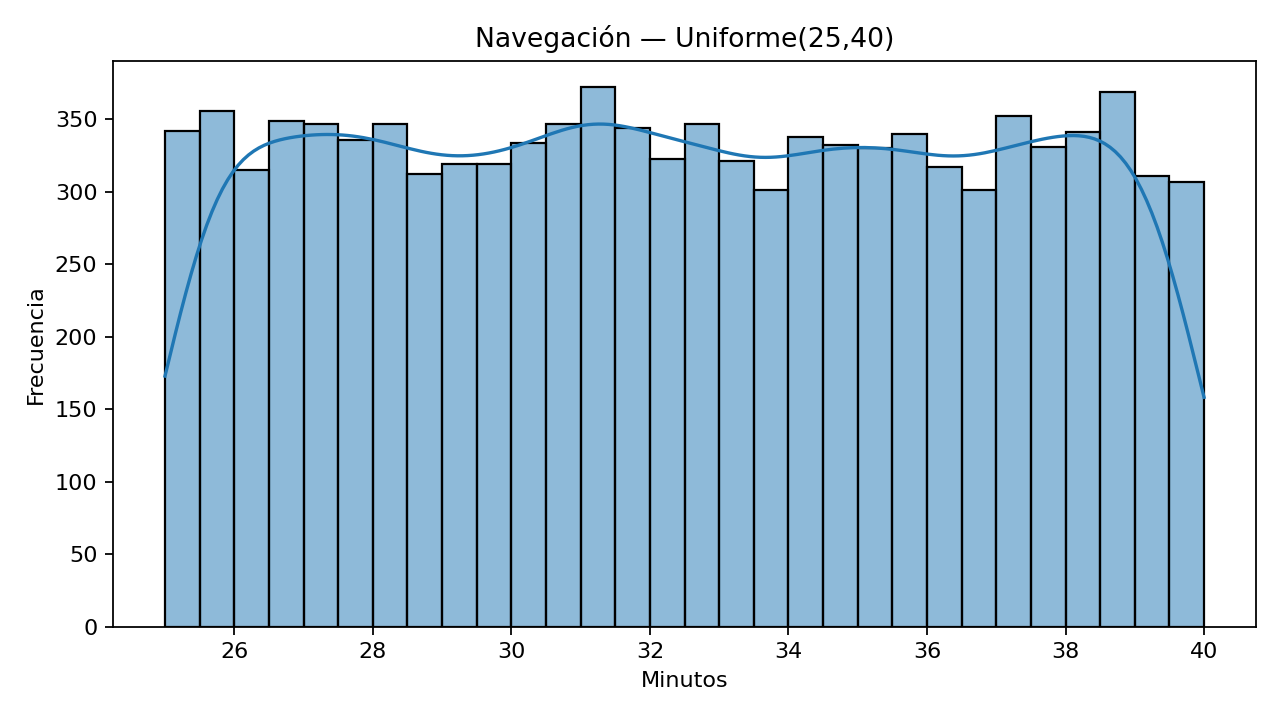
\includegraphics[width=\textwidth]{../figures/hist_navegacion.png}
    \caption{Navegación -- Uniforme}
  \end{subfigure}

  \vspace{0.5cm}

  \begin{subfigure}[b]{0.48\textwidth}
    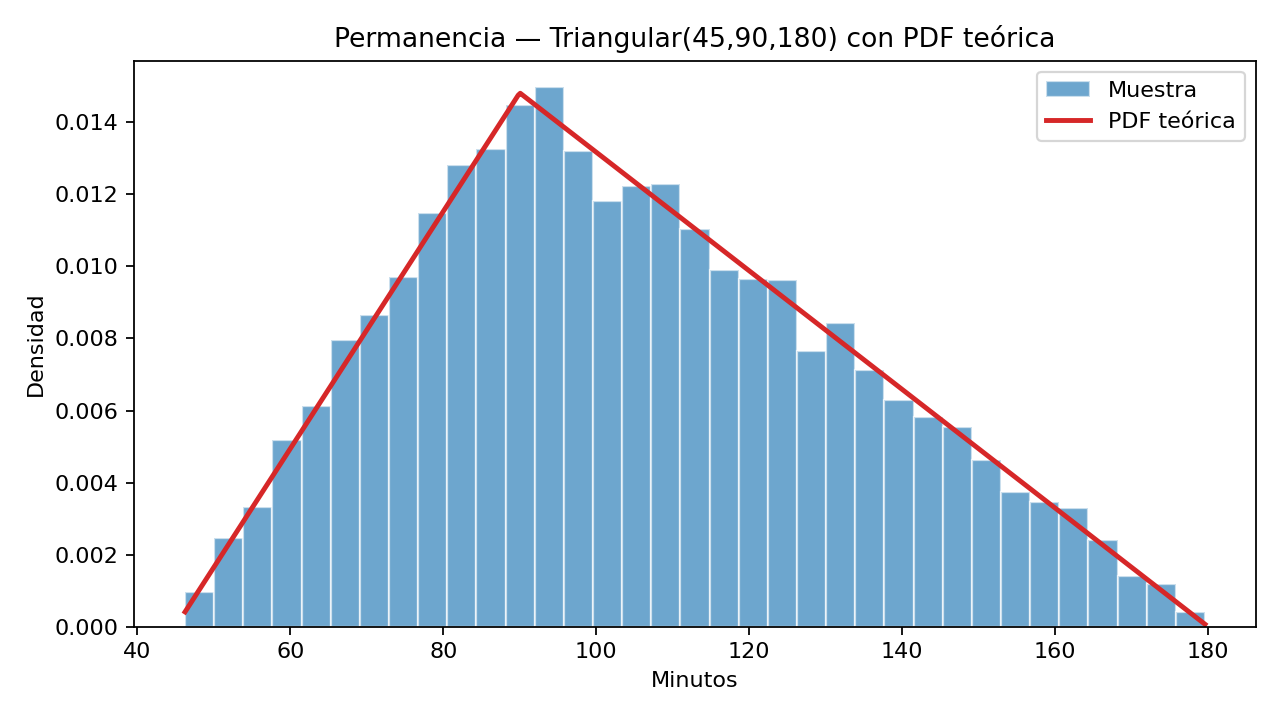
\includegraphics[width=\textwidth]{../figures/hist_permanencia.png}
    \caption{Permanencia -- Triangular}
  \end{subfigure}

  \caption{Histogramas de validación (10\,000 muestras cada uno)}
\end{figure}

% -----------------------------------------------------------------------
% 12. RESULTADOS DEL ESCENARIO BASE
% -----------------------------------------------------------------------
\section{Resultados del escenario base}

Los resultados corresponden al promedio de 1\,000 réplicas Montecarlo con
semilla~2026. La jornada simula 240 minutos de llegadas desde las 06:00
hasta las 10:00.

\begin{table}[H]
  \centering
  \caption{Métricas del escenario base (E0) -- promedio de 1\,000 réplicas}
  \begin{tabular}{@{}lr@{}}
    \toprule
    Métrica & Valor promedio \\
    \midrule
    Espera promedio ($W_q$)            & 66,21 min \\
    Tiempo promedio en sistema ($W$)   & 236,43 min \\
    Longitud promedio de cola ($L_q$)  & 8,83 grupos \\
    Utilización de embarcaciones       & 82,8\% \\
    Porcentaje que espera en cola      & 87,5\% \\
    Percentil 95 de espera             & 142,72 min \\
    Turistas atendidos por jornada     & 119,9 \\
    Turistas no atendidos por jornada  & 224,9 \\
    Viajes realizados                  & 5,2 \\
    Ocupación promedio por viaje       & 77,2\% \\
    \bottomrule
  \end{tabular}
\end{table}

\subsection{Interpretación}

El ciclo promedio de una embarcación es de aproximadamente 180 minutos
(32,5 + 105 + 32,5 + 10). Con 3 embarcaciones operando en una jornada de
240 minutos, cada embarcación puede completar entre 1 y 2 viajes completos.
Esto limita la capacidad efectiva a aproximadamente 120--160 turistas,
mientras que la demanda promedio es de alrededor de 345 turistas por
jornada (8 grupos/hora × 4 horas × 10,6 turistas/grupo).

El sistema está \textbf{estructuralmente congestionado}: incluso sin
variabilidad, la capacidad es insuficiente para la demanda. La espera
promedio de 66 minutos y el percentil 95 de 143 minutos confirman que una
fracción significativa de grupos experimenta esperas largas antes de
abordar.

% -----------------------------------------------------------------------
% 13. COMPARACIÓN DE ESCENARIOS
% -----------------------------------------------------------------------
\section{Comparación de escenarios}

Para que la simulación tenga valor práctico, no basta con analizar un
solo caso. Se diseñaron cuatro escenarios alternativos al base con el
objetivo de responder una pregunta concreta: ¿qué cambio operativo
mejora más el sistema con menor costo de implementación?

Los cinco escenarios evaluados son:

\begin{itemize}[noitemsep]
  \item \textbf{E0 — Base:} 3 embarcaciones, capacidad 30 turistas,
    preparación 10 min, demanda de 8 grupos/hora.
  \item \textbf{E1 — Más embarcaciones:} se agrega una cuarta
    embarcación manteniendo todo lo demás igual.
  \item \textbf{E2 — Menor preparación:} se reduce el tiempo de
    alistamiento de 10 a 5 minutos entre viajes.
  \item \textbf{E3 — Mayor capacidad:} las embarcaciones pasan de 30
    a 40 turistas de capacidad, con umbral de salida en 32.
  \item \textbf{E4 — Alta demanda:} la tasa de llegada sube a 10
    grupos por hora, simulando un día de mayor afluencia.
\end{itemize}

\begin{table}[H]
  \centering
  \caption{Comparación de escenarios -- promedio de 1\,000 réplicas
    Montecarlo}
  \small
  \begin{tabular}{@{}lrrrrrr@{}}
    \toprule
    Escenario & Espera & $L_q$ & Util. & Percentil 95 & Atend. &
      No atend. \\
              & (min)  & (gr.) & (\%)  & (min)        &        & \\
    \midrule
    E0 Base              & 66,21 &  8,83 & 82,8 & 142,72 & 119,9 & 224,9 \\
    E1 Más embarcaciones & 55,65 &  7,42 & 79,3 & 126,51 & 149,6 & 190,0 \\
    E2 Menor preparación & 66,16 &  8,82 & 82,7 & 140,19 & 121,8 & 219,0 \\
    E3 Mayor capacidad   & 61,77 &  8,24 & 80,8 & 129,25 & 148,0 & 192,5 \\
    E4 Alta demanda      & 71,85 & 11,98 & 84,5 & 154,79 & 125,7 & 304,4 \\
    \bottomrule
  \end{tabular}
\end{table}

\subsection{Gráficos comparativos}

\begin{figure}[H]
  \centering
  \begin{subfigure}[b]{0.48\textwidth}
    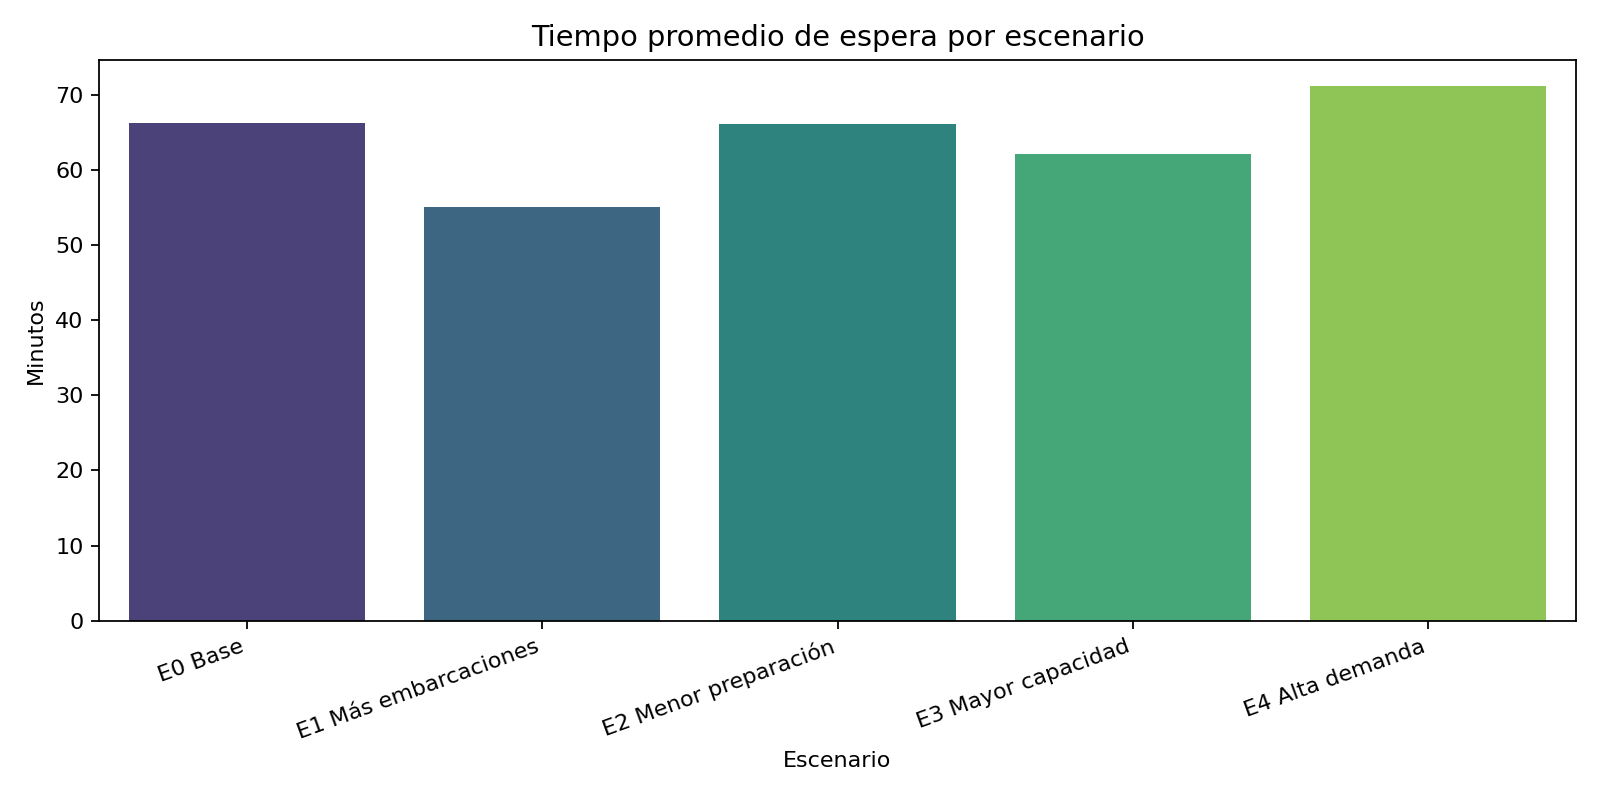
\includegraphics[width=\textwidth]{../figures/escenarios_espera_promedio.png}
    \caption{Espera promedio por escenario}
  \end{subfigure}
  \hfill
  \begin{subfigure}[b]{0.48\textwidth}
    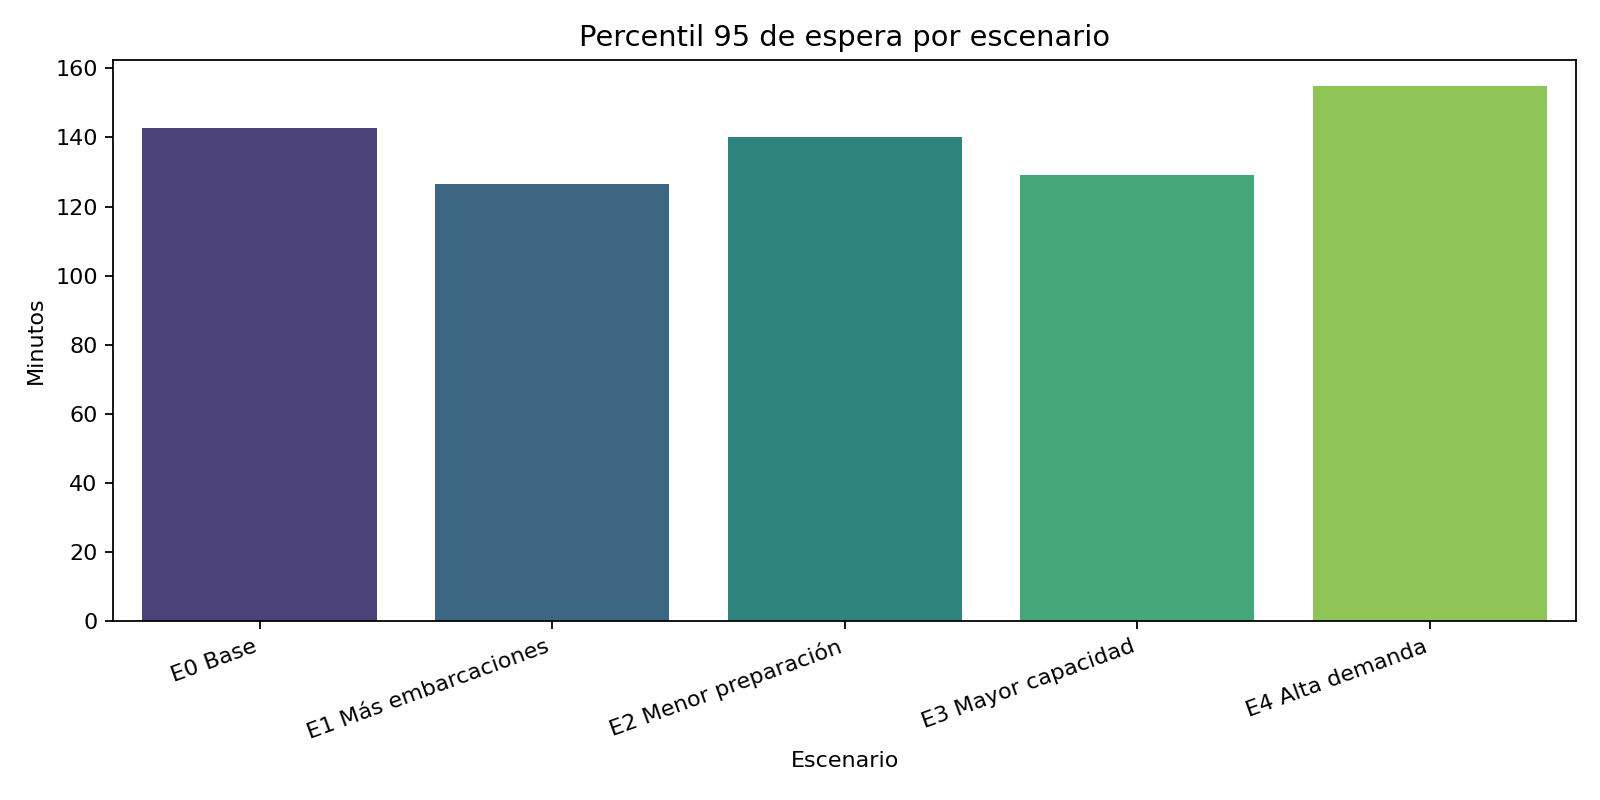
\includegraphics[width=\textwidth]{../figures/escenarios_percentil95.png}
    \caption{Percentil 95 de espera}
  \end{subfigure}

  \vspace{0.5cm}

  \begin{subfigure}[b]{0.48\textwidth}
    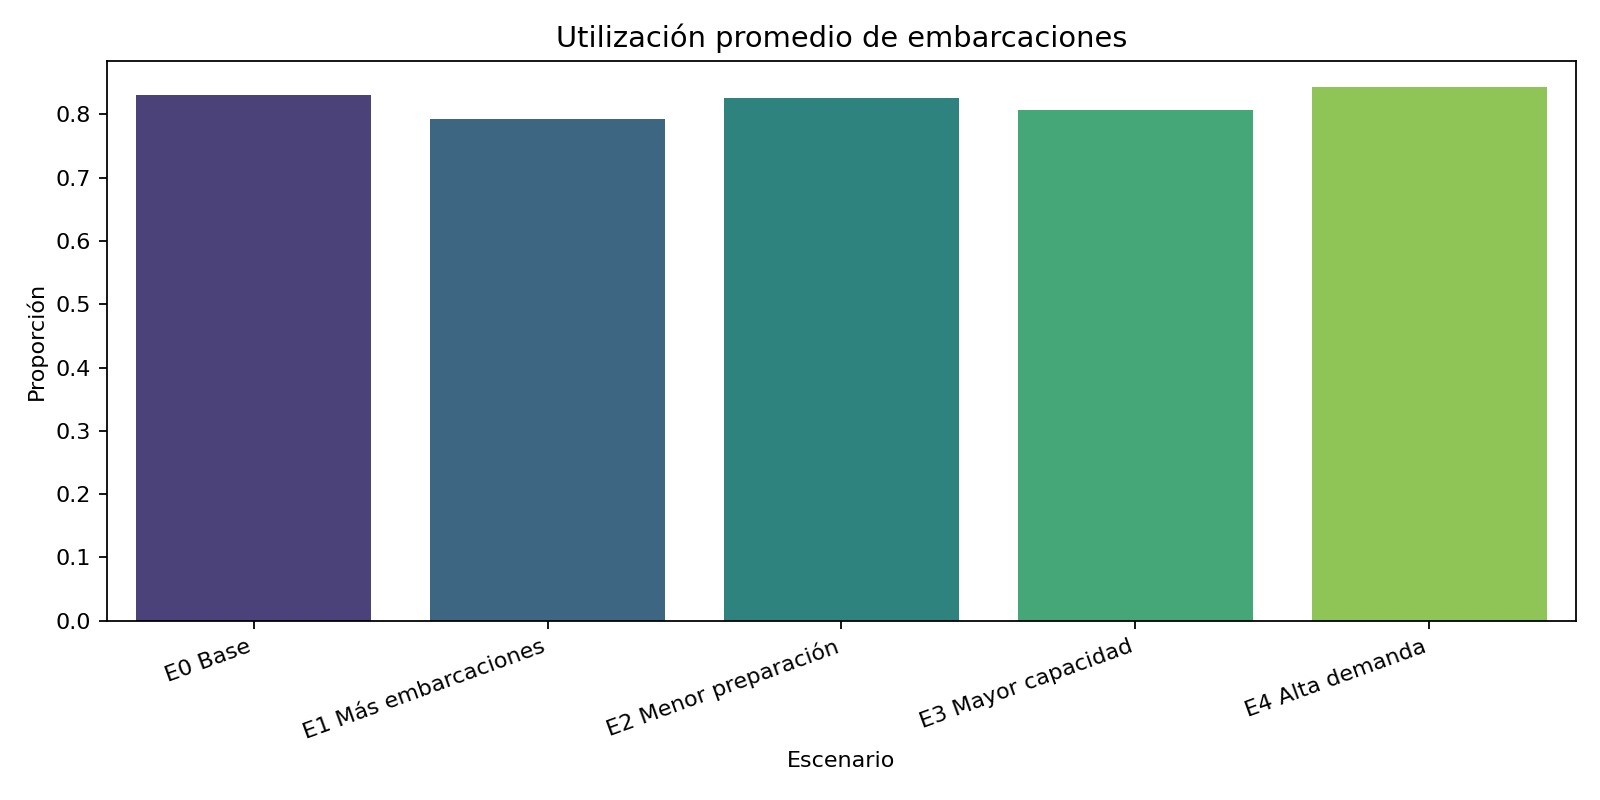
\includegraphics[width=\textwidth]{../figures/escenarios_utilizacion.png}
    \caption{Utilización de embarcaciones}
  \end{subfigure}
  \hfill
  \begin{subfigure}[b]{0.48\textwidth}
    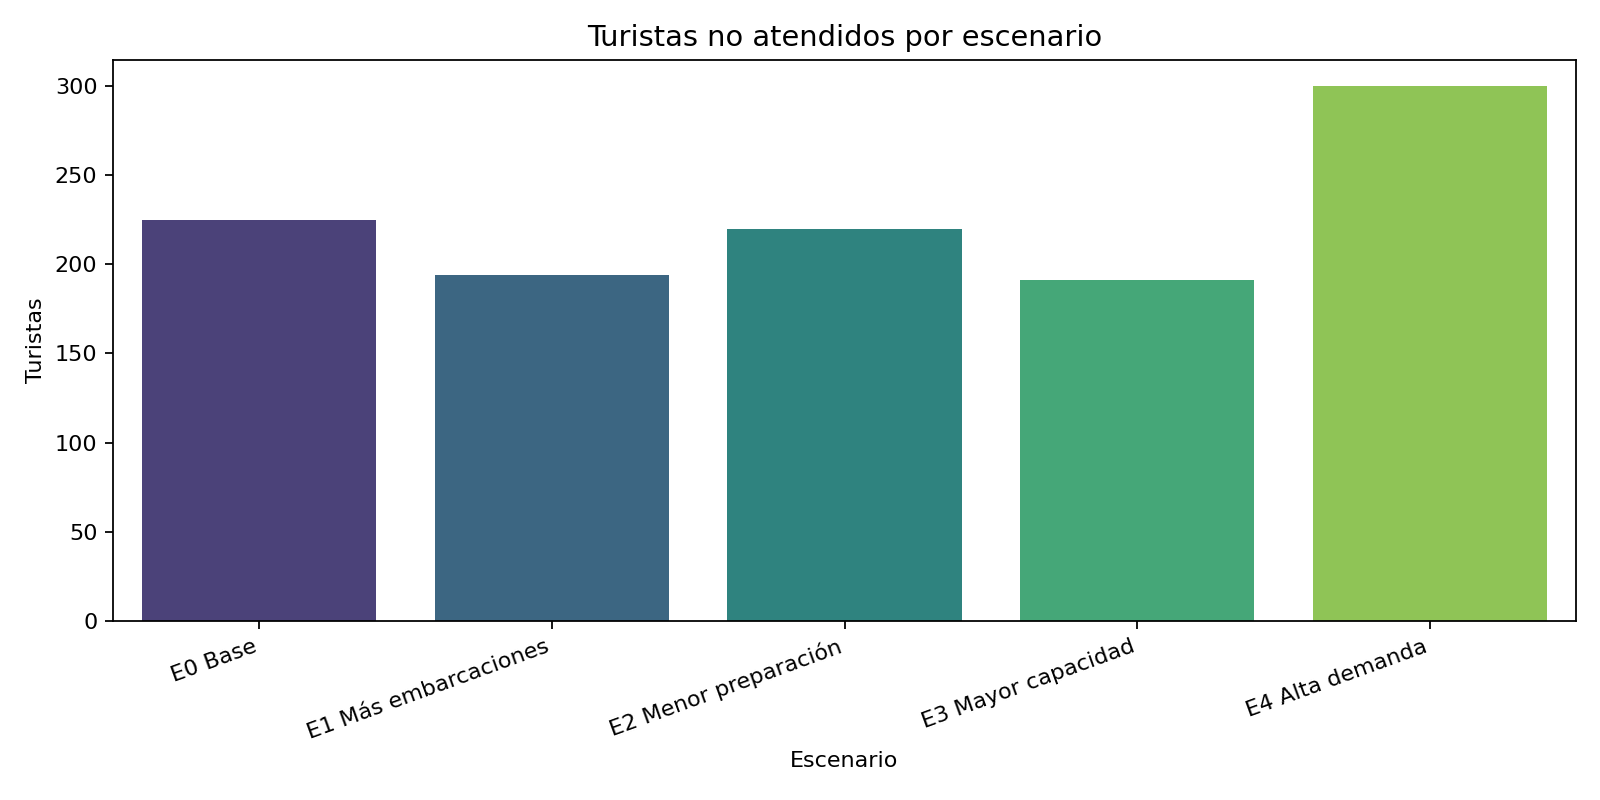
\includegraphics[width=\textwidth]{../figures/escenarios_turistas_no_atendidos.png}
    \caption{Turistas no atendidos}
  \end{subfigure}

  \caption{Comparación de métricas entre escenarios E0--E4}
\end{figure}

\subsection{Análisis de resultados por escenario}

\paragraph{E0 — Base.}
El sistema opera con una espera promedio de 66,21 minutos y una
utilización del 82,8\%. El percentil 95 de espera llega a 142,72
minutos, lo que significa que 1 de cada 20 grupos espera más de dos
horas y media solo para embarcar. Eso evidencia un sistema con
congestión real, no marginal.

\paragraph{E1 — Más embarcaciones.}
Agregar una cuarta embarcación reduce la espera promedio en 10,56
minutos y el percentil 95 baja a 126,51 minutos. Los turistas
atendidos suben de 119,9 a 149,6, un incremento del 24,7\%. Es la
mejora más grande en términos absolutos, pero también la que mayor
inversión requiere: una embarcación adicional implica compra,
matrícula, tripulación y mantenimiento.

\paragraph{E2 — Menor preparación.}
Este es el resultado más revelador del análisis. Reducir el tiempo
de preparación de 10 a 5 minutos, exactamente a la mitad, produce
una mejora de apenas \textbf{0,05 minutos} en la espera promedio.
Prácticamente nada. La razón es matemáticamente clara: la preparación
representa solo el 5,6\% del ciclo total de 180 minutos. Ahorrar 5
minutos por viaje, en 5,2 viajes promedio por jornada, da un ahorro
total de 26 minutos distribuidos entre 3 embarcaciones, insuficiente
para liberar capacidad real. Optimizar ese proceso no está justificado
por los resultados.

\paragraph{E3 — Mayor capacidad.}
Aumentar la capacidad a 40 turistas por embarcación reduce la espera
a 61,77 minutos y el percentil 95 a 129,25 minutos. Los turistas
atendidos llegan a 148,0, casi igual que en E1 pero sin agregar
ninguna embarcación nueva. Es un resultado relevante porque logra
un impacto comparable a E1 a través de un cambio operativo diferente:
embarcaciones más grandes en lugar de más embarcaciones.

\paragraph{E4 — Alta demanda.}
Con 10 grupos por hora el sistema se deteriora notablemente: 304,4
turistas no atendidos por jornada, un 35\% más que en el escenario
base. Este escenario no representa una mejora sino una prueba de
estrés que confirma algo importante: el sistema ya opera cerca de su
límite. Un incremento de demanda moderado lo desborda por completo.

% -----------------------------------------------------------------------
% 14. DISCUSIÓN
% -----------------------------------------------------------------------
\section{Discusión}

\subsection{Lo que E2 revela sobre el verdadero cuello de botella}

Uno podría asumir que si se reduce el tiempo muerto entre viajes, el
sistema debería mejorar. Los números dicen lo contrario. El tiempo de
preparación de 10 minutos parece significativo cuando se observa un
solo viaje, pero dentro del ciclo completo de 180 minutos representa
apenas el 5,6\%. Reducirlo a 5 minutos ahorra 26 minutos totales
distribuidos entre 3 embarcaciones en toda la jornada, un valor
demasiado pequeño para generar un viaje adicional o reducir la cola
de forma perceptible.

Esto confirma que el cuello de botella no está en la preparación sino
en la relación entre la capacidad de la flota y el volumen de demanda.
El sistema recibe alrededor de 345 turistas por jornada pero solo puede
transportar entre 120 y 160. Esa brecha estructural no se cierra con
ajustes menores.

\subsection{Por qué E1 funciona mejor que todos}

Agregar una embarcación aumenta la capacidad del sistema en un 33\%.
Más importante aún, la cuarta embarcación opera en paralelo con las
otras tres, lo que significa que puede completar su ciclo mientras las
demás aún están en viaje. Eso se traduce directamente en más grupos
atendidos antes del cierre de la jornada: de 119,9 a 149,6 turistas
promedio, con 35 turistas no atendidos menos por día. El percentil 95
de espera cae 16 minutos. Es la intervención con mayor impacto
numérico en todas las métricas.

\subsection{Por qué E3 es una alternativa real}

Lo interesante de E3 es que logra resultados muy cercanos a E1 sin
ampliar la flota. Pasar de 30 a 40 turistas por embarcación permite
que cada viaje sea más productivo: se transportan más personas por
ciclo con el mismo número de botes. Los turistas atendidos llegan a
148, casi idéntico a los 149,6 de E1. La diferencia práctica es que
E3 requiere embarcaciones de mayor porte o capacidad ampliada, lo que
puede ser más fácil de gestionar operativamente que adquirir una
unidad completamente nueva.

\subsection{Lo que E4 anticipa}

El escenario de alta demanda no es una mejora sino una advertencia.
Si la demanda sube apenas un 25\% (de 8 a 10 grupos por hora), el
sistema pasa de 224,9 turistas no atendidos a 304,4. Un incremento
del 35\% en turistas no atendidos por un aumento del 25\% en demanda.
Esa desproporción indica que el sistema no tiene margen de absorción.
Ante cualquier evento que concentre más turistas en el muelle, como
festividades o feriados, el sistema colapsará sin una intervención
estructural previa.

% -----------------------------------------------------------------------
% 15. CONCLUSIONES
% -----------------------------------------------------------------------
\section{Conclusiones}

A partir de los resultados obtenidos en las 1\,000 réplicas Montecarlo
por escenario, se pueden establecer las siguientes conclusiones:

\begin{enumerate}[noitemsep]
  \item Se identificaron cinco variables aleatorias con variabilidad
    relevante para el sistema: tiempo entre llegadas, tamaño de grupo,
    tiempo de registro, tiempo de navegación y tiempo de permanencia
    en isla.
  \item Las distribuciones Exponencial, Triangular y Uniforme modelan
    adecuadamente cada variable. La validación con 10\,000 muestras
    mostró desviaciones inferiores al 1\% respecto a las medias
    teóricas en todos los casos.
  \item La ficha de observación sintética, construida con base en
    fuentes públicas y el PDF del trabajo, permite justificar los
    parámetros del modelo de forma académicamente coherente sin
    necesidad de datos de campo propios.
  \item El escenario base evidencia que el sistema está estructuralmente
    congestionado: la demanda promedio supera la capacidad efectiva en
    aproximadamente el 65\% de los turistas por jornada.
  \item La simulación Montecarlo con 1\,000 réplicas produce resultados
    estables y reproducibles. Los promedios no cambian de forma
    significativa al aumentar el número de réplicas, lo que confirma
    la convergencia del método.
  \item Reducir el tiempo de preparación (E2) no mejora el sistema de
    manera perceptible porque ese tiempo no es el cuello de botella.
  \item Aumentar la capacidad por embarcación (E3) y agregar una
    embarcación (E1) son las únicas intervenciones que producen mejoras
    reales y medibles en todas las métricas.
  \item El escenario de alta demanda (E4) confirma que el sistema no
    tiene capacidad de absorción ante incrementos de afluencia. Se
    requieren mejoras estructurales antes de que eso ocurra.
\end{enumerate}

% -----------------------------------------------------------------------
% 16. RECOMENDACIONES
% -----------------------------------------------------------------------
\section{Recomendaciones}

Con base en los criterios de menor espera, menor demanda no atendida,
utilización en rango aceptable (70--90\%) y factibilidad operativa:

\begin{description}
  \item[Recomendación primaria -- E1:] Incorporar una cuarta embarcación.
    Es la mejora con mayor impacto en turistas atendidos (+24,7\%) y mayor
    reducción de la espera promedio (--16,0\%). La utilización baja a 79,3\%,
    lo que deja margen para días de mayor demanda.

  \item[Alternativa de eficiencia -- E3:] Si adquirir un bote nuevo no es
    viable, reemplazar las embarcaciones actuales por unidades de 40
    turistas de capacidad ofrece resultados comparables (148 atendidos,
    192 no atendidos) con el mismo número de botes.

  \item[No recomendado -- E2:] Reducir el tiempo de preparación produce
    una mejora prácticamente nula ($<0{,}1$ min de espera promedio). La
    inversión en optimización de ese proceso no está justificada por los
    resultados del modelo.

  \item[Planificación ante alta demanda:] Si se prevén periodos con $>8$
    grupos/hora (festividades, feriados), se recomienda implementar E1
    con carácter permanente y activar una embarcación de reserva adicional.
\end{description}

% -----------------------------------------------------------------------
% 17. REFERENCIAS
% -----------------------------------------------------------------------
\section{Referencias}

\begin{enumerate}[label={[\arabic*]}, noitemsep]
  \item Ministerio de Comercio Exterior y Turismo (MINCETUR). (2026).
    \textit{Festividad Virgen de la Candelaria 2026 -- Estadísticas de
    turismo receptivo Puno}. Lima: MINCETUR. Recuperado de
    \url{https://www.mincetur.gob.pe}

  \item Ministerio de Comercio Exterior y Turismo (MINCETUR). (2024).
    \textit{Ente Gestor Destino Lago Titicaca}. Lima: MINCETUR. Recuperado
    de \url{https://www.mincetur.gob.pe}

  \item Servicio Nacional de Áreas Naturales Protegidas por el Estado
    (SERNANP). (2024). \textit{Reserva Nacional del Titicaca}. Lima:
    SERNANP. Recuperado de \url{https://www.sernanp.gob.pe}

  \item PunoTours. (2026). \textit{Tour Islas Uros y Taquile -- Full Day}.
    Puno: PunoTours. Recuperado de \url{https://www.punotours.pe}

  \item Harris, C. R., et al. (2020). Array programming with NumPy.
    \textit{Nature}, 585, 357--362.
    \url{https://doi.org/10.1038/s41586-020-2649-2}

  \item McKinney, W. (2010). Data structures for statistical computing in
    Python. \textit{Proceedings of the 9th Python in Science Conference},
    51--56.

  \item Hunter, J. D. (2007). Matplotlib: A 2D graphics environment.
    \textit{Computing in Science \& Engineering}, 9(3), 90--95.

  \item Waskom, M. L. (2021). Seaborn: Statistical data visualization.
    \textit{Journal of Open Source Software}, 6(60), 3021.
    \url{https://doi.org/10.21105/joss.03021}
\end{enumerate}

% -----------------------------------------------------------------------
% 18. ANEXOS
% -----------------------------------------------------------------------
\section{Anexos}

\subsection{Anexo A -- Función de simulación de una jornada}

\begin{lstlisting}[caption={Función \texttt{simular\_jornada}}]
def simular_jornada(rng, duracion=240, lambda_grupos=8,
                    n_embarcaciones=3, capacidad=30,
                    t_prep=10, umbral=24, espera_max=15):
    cola = generar_grupos(rng, duracion, lambda_grupos)
    cola.sort(key=lambda g: g["fin_reg"])
    botes = [0.0] * n_embarcaciones
    esperas, sistemas, esperas_cola = [], [], []
    viajes = 0; atendidos = 0; ocupado = 0.0

    while cola:
        bote_idx = int(np.argmin(botes))
        t_inicio = max(botes[bote_idx], cola[0]["fin_reg"])
        if t_inicio > duracion:
            break   # jornada cerrada; restantes = no atendidos
        t = t_inicio
        carga, cargados, i = 0, [], 0
        limite = cola[0]["fin_reg"] + espera_max

        while i < len(cola):
            g = cola[i]
            if g["fin_reg"] > max(t, limite): break
            t = max(t, g["fin_reg"])
            if carga + g["tamano"] <= capacidad:
                carga += g["tamano"]; cargados.append(g); i += 1
                if carga >= umbral: break
            else: break

        if not cargados:
            botes[bote_idx] = cola[0]["fin_reg"]; continue

        salida = t if carga >= umbral else max(t, limite)
        if salida > duracion: break  # no parte tras cierre

        ciclo_sin = (rng.uniform(25,40) +
                     rng.triangular(45,90,180) +
                     rng.uniform(25,40))
        ciclo = ciclo_sin + t_prep
        ocupado += min(salida + ciclo, duracion) - salida
        botes[bote_idx] = salida + ciclo
        viajes += 1; atendidos += carga

        for g in cargados:
            espera = salida - g["t_llegada"]
            esperas.append(espera)
            esperas_cola.append(max(0., salida - g["fin_reg"]))
            sistemas.append(espera + ciclo_sin)
        cola = cola[len(cargados):]

    no_atendidos = sum(g["tamano"] for g in cola)
    ...
\end{lstlisting}

\subsection{Anexo B -- Parámetros de los escenarios}

\begin{table}[H]
  \centering
  \caption{Configuración de cada escenario}
  \begin{tabular}{@{}llrrrrr@{}}
    \toprule
    Código & Nombre & $\lambda$ (gr/h) & Emb. & Cap. & Umbral & Prep. \\
    \midrule
    E0 & Base               & 8  & 3 & 30 & 24 & 10 min \\
    E1 & Más embarcaciones  & 8  & 4 & 30 & 24 & 10 min \\
    E2 & Menor preparación  & 8  & 3 & 30 & 24 &  5 min \\
    E3 & Mayor capacidad    & 8  & 3 & 40 & 32 & 10 min \\
    E4 & Alta demanda       & 10 & 3 & 30 & 24 & 10 min \\
    \bottomrule
  \end{tabular}
\end{table}

% =======================================================================
\end{document}
% =======================================================================
